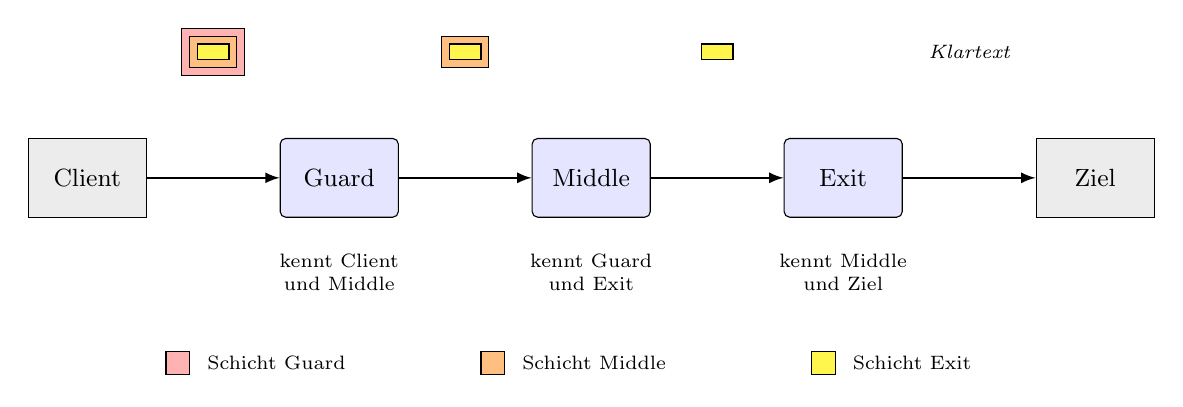
\begin{tikzpicture}[
    >=latex,
    every node/.style={font=\small},
    relay/.style={
        draw, rounded corners=2pt,
        minimum width=15mm, minimum height=10mm,
        align=center, fill=blue!10
    },
    endpoint/.style={
        draw,
        minimum width=15mm, minimum height=10mm,
        align=center, fill=gray!15
    }
]

\def\dx{32mm}

% Main row of nodes: Client - Guard - Middle - Exit - Ziel
\node[endpoint] (c0) at (0*\dx, 0) {Client};
\node[relay]    (n1) at (1*\dx, 0) {Guard};
\node[relay]    (n2) at (2*\dx, 0) {Middle};
\node[relay]    (n3) at (3*\dx, 0) {Exit};
\node[endpoint] (c1) at (4*\dx, 0) {Ziel};

% Arrows between nodes
\draw[->, thick] (c0) -- (n1);
\draw[->, thick] (n1) -- (n2);
\draw[->, thick] (n2) -- (n3);
\draw[->, thick] (n3) -- (c1);

% Encryption layers above each arrow (the shrinking onion)
% Hop 1 (Client -> Guard): three layers
\fill[red!30]    (0.5*\dx-4mm, 13mm) rectangle ++(8mm, 6mm);
\draw            (0.5*\dx-4mm, 13mm) rectangle ++(8mm, 6mm);
\fill[orange!50] (0.5*\dx-3mm, 14mm) rectangle ++(6mm, 4mm);
\draw            (0.5*\dx-3mm, 14mm) rectangle ++(6mm, 4mm);
\fill[yellow!70] (0.5*\dx-2mm, 15mm) rectangle ++(4mm, 2mm);
\draw            (0.5*\dx-2mm, 15mm) rectangle ++(4mm, 2mm);

% Hop 2 (Guard -> Middle): two layers
\fill[orange!50] (1.5*\dx-3mm, 14mm) rectangle ++(6mm, 4mm);
\draw            (1.5*\dx-3mm, 14mm) rectangle ++(6mm, 4mm);
\fill[yellow!70] (1.5*\dx-2mm, 15mm) rectangle ++(4mm, 2mm);
\draw            (1.5*\dx-2mm, 15mm) rectangle ++(4mm, 2mm);

% Hop 3 (Middle -> Exit): one layer
\fill[yellow!70] (2.5*\dx-2mm, 15mm) rectangle ++(4mm, 2mm);
\draw            (2.5*\dx-2mm, 15mm) rectangle ++(4mm, 2mm);

% Hop 4 (Exit -> Ziel): plaintext
\node[font=\scriptsize\itshape] at (3.5*\dx, 16mm) {Klartext};

% Annotations under each relay (what each node knows)
\node[font=\scriptsize, align=center, text width=26mm] at (1*\dx, -12mm)
    {kennt Client\\und Middle};
\node[font=\scriptsize, align=center, text width=26mm] at (2*\dx, -12mm)
    {kennt Guard\\und Exit};
\node[font=\scriptsize, align=center, text width=26mm] at (3*\dx, -12mm)
    {kennt Middle\\und Ziel};

% Legend
\fill[red!30]    (10mm, -25mm) rectangle ++(3mm, 3mm);
\draw            (10mm, -25mm) rectangle ++(3mm, 3mm);
\node[font=\scriptsize, anchor=west] at (14mm, -23.5mm) {Schicht Guard};

\fill[orange!50] (50mm, -25mm) rectangle ++(3mm, 3mm);
\draw            (50mm, -25mm) rectangle ++(3mm, 3mm);
\node[font=\scriptsize, anchor=west] at (54mm, -23.5mm) {Schicht Middle};

\fill[yellow!70] (92mm, -25mm) rectangle ++(3mm, 3mm);
\draw            (92mm, -25mm) rectangle ++(3mm, 3mm);
\node[font=\scriptsize, anchor=west] at (96mm, -23.5mm) {Schicht Exit};

\end{tikzpicture}
